\subsection{Cơ sở dữ liệu (Database)}
\subsubsection{Hệ cơ sở dữ liệu quan hệ (RDBMS)}
\textbf{Khái niệm:}\\

RDBMS - Relational Database Management System - là hệ cơ sở dữ liệu quan hệ. Tất cả các hệ thống quản trị cơ sở dữ liệu hiện đại như SQL, MySQL, MS SQL Server, Oracle, ... đều dựa trên RDBMS.

Hệ thống quản lý cơ sở dữ liệu quan hệ (RDBMS) là một hệ thống quản lý cơ sở dữ liệu (DBMS) dựa trên mô hình quan hệ được giới thiệu bởi EF Codd.

\textbf{Bảng (Table):}\\

RDBMS sử dụng các bảng để lưu trữ dữ liệu. Mỗi bảng là một tập hợp các dữ liệu có liên quan đến nhau và có nhiều hàng và cột để lưu dữ liệu. Bảng là hình thức lưu trữ phổ biến và đơn giản nhất trong môt cơ sở dữ liệu quan hệ. Ví dụ về bảng một nhóm môn học trong bảng MONHOC sau đây:\\
\begin{table}[H]
    \centering
    \begin{tabular}{|l|l|l|}
    \hline
         \textbf{ID}&\textbf{TEN\_MON\_HOC}&\textbf{SO\_TIN\_CHI}\\
         \hline
         1&Giải tích 1&4\\
		\hline
		2&Vật lý&3\\
		\hline			
		3&Kỹ thuật lập trình&4\\
		\hline
    \end{tabular}
    \caption{Ví dụ về bảng dữ liệu}
\end{table}

\textbf{Trường (Field):}\\
	
	Mỗi bảng được chia thành các thực thể nhỏ gọi là các trường, chứa các thông tin cụ thể về mỗi bản ghi trong bảng. Các trường trong bảng MONHOC bao gồm: ID, TEN\_MON\_HOC, SO\_TIN\_CHI.\\
	\begin{table}[H]
	    \centering
	    \begin{tabular}{|l|}
	        \hline
	        \textbf{TEN\_MON\_HOC}\\
	        \hline
	        Giải tích 1\\
	        \hline
	        Vật lý\\
	        \hline
	        Kỹ thuật lập trình\\
	        \hline
	    \end{tabular}
	    \caption{Ví dụ một trường trong bảng dữ liệu}
	\end{table}
	
\textbf{Hàng hoặc bản ghi (Record):}\\
	
Một hàng của bảng được gọi là bản ghi , nó chứa thông tin của một đối tượng trong bảng. Ví dụ ở bảng MONHOC có 3 bản ghi. Sau đây là một bản ghi trong bảng:\\
\begin{table}[H]
    \centering
    \begin{tabular}{|r|r|r|}
        \hline
		1&Giải tích 1&4\\
		\hline
    \end{tabular}
    \caption{Ví dụ về một bản ghi}
\end{table}

\textbf{Ràng buộc (Constraint):}

Ràng buộc là các quy tắc cho các cột dữ liệu trong bảng. Chúng được sử dụng để giới hạn loại dữ liệu có thể insert vào một bảng. Điều này đảm bảo tính chính xác và độ tin cậy của dữ liệu trong cơ sở dữ liệu.\\
Constraint có thể là cấp độ cột hoặc cấp độ bảng. Các ràng buộc cấp độ cột chỉ được áp dụng cho một
cột trong khi các ràng buộc mức bảng được áp dụng cho toàn bộ bảng.\\
Sau đây là một số ràng buộc phổ biến nhất được sử dụng trong SQL :\\
\begin{table}[H]
    \centering
    \begin{tabular}{|l|l|}
        \hline
         NOT NULL&Đảm bảo rằng một field không có giá trị NULL  \\
         \hline
         DEFAULT&Cung cấp giá trị mặc định của một field khi không được xác định\\
         \hline
         UNIQUE&Đảm bảo giá trị trong một field là khác nhau\\
         \hline
         PRIMARY Key&Mỗi record là duy nhất trong một bảng cơ sở dữ liệu\\
         \hline
         FOREIGN Key&Mỗi record là duy nhất trong trong bất kỳ bảng cơ sở dữ liệu khác\\
         \hline
         CHECK&Đảm bảo rằng tất cả các giá trị trong một cột thỏa mãm một số điều kiện\\
         \hline
         INDEX&Dùng để tạo và lấy dữ liệu một cách nhanh chóng\\
         \hline
    \end{tabular}
    \caption{Một số ràng buộc phổ biến trong SQL}
\end{table}
\subsubsection{Hệ quản trị cơ sở dữ liệu}

Hệ quản trị cơ sở dữ liệu (Database Management System - DBMS) là hệ thống kiểm soát việc lưu trữ, tổ chức và truy xuất dữ liệu.

Mỗi DBMS đều có thành phần gọi là Query Language (Ngôn ngữ truy vấn), các ứng dụng muốn truy cập dữ liệu đều phải nhờ vào thành phần này.

Các hệ quản trị cơ sở dữ liệu quan hệ phổ biến nhất hiện nay:
\subsubsubsection{Oracle Database}
\begin{center}
  \captionsetup{type=figure}
  
\includegraphics[scale=0.4]{img/oracle.jpg}
  \captionof{figure}{Oracle Database}
\end{center}

Oracle Database hay còn gọi là Oracle RDBMS hoặc đơn giản là Oracle là 1 hệ quản trị cơ sở dữ liệu quan hệ, được phát triển và phân phối bởi tập đoàn Oracle.

\textit{Đặc điểm và thế mạnh:}
\begin{itemize}
    \item Quản lý được hệ thống dữ liệu lớn
    \item Hỗ trợ nhiều công cụ để quản trị cũng như nhập, xuất dữ liệu dễ dàng
    \item Có thể hoạt động trên nhiều hệ điều hành khác nhau như Windows, Linux, Mac OS, Unix,...
    \item Truy cập đồng thời
    \item Hỗ trợ cơ chế khóa
    \item Thực thi song song
    \item Tính khả chuyển
\end{itemize}

\subsubsubsection{MySQL}
\begin{center}
  \captionsetup{type=figure}
    
\includegraphics[scale=0.5]{img/mysql.jpg}
  \captionof{figure}{MySQL}
\end{center}

MySQL là một hệ quản trị cơ sở dữ liệu quan hệ mã nguồn mở, được phát triển, phân phối và hỗ trợ bởi tập đoàn Oracle.\\

\textit{Đặc điểm và thế mạnh:}
\begin{itemize}
    \item \textbf{Tính nội bộ và linh động:}
    \begin{itemize}
    \item Viết bằng C và C++
    \item Đã thử nghiệm với một loạt các trình biên dịch khác nhau
    \item Hoạt động trên nhiều nền tảng khác nhau
    \item Sử dụng thiết kế máy chủ nhiều lớp với các mo-đun độc lập
    \item Được thiết kế để đa luồng hoàn toàn bằng cách sử dụng các luồng nhân, để dễ dàng sử dụng nhiều CPU nếu chúng có sẵn
    \item Triển khai các bảng băm trong bộ nhớ, được sử dụng làm bảng tạm thời.
    \item Triển khai các hàm SQL bằng cách sử dụng thư viện lớp được tối ưu hóa cao nhất phải nhanh nhất có thể
    \end{itemize}
    \item \textbf{Bảo mật}
    \begin{itemize}
        \item Một hệ thống đặc quyền và mật khẩu rất linh hoạt và an toàn, và cho phép xác minh dựa trên máy chủ
        \item Bảo mật mật khẩu bằng cách mã hóa tất cả lưu lượng mật khẩu khi bạn kết nối với máy chủ.
    \end{itemize}
    \item \textbf{Khả năng mở rộng và giới hạn:}
    \begin{itemize}
        \item Hỗ trợ cơ sở dữ liệu lớn
        \item Hỗ trợ lên đến 64 chỉ mục cho mỗi bảng
    \end{itemize}
    \item \textbf{Ổn định, có tốc độ cao và dễ sử dụng}
    \item \textbf{Đa tính năng:} Hỗ trợ rất nhiều chức năng SQL
\end{itemize}
\subsubsubsection{SQL Server}
\begin{center}
  \captionsetup{type=figure}
    
\includegraphics[scale=0.3]{img/sql-server.png}
  \captionof{figure}{SQL Server}
\end{center}
SQL Server là một RDBMS được phát triển bởi tập đoàn Microsoft.

\textit{Thế mạnh:}
\begin{itemize}
    \item Cho phép nhiều người dùng chung một cơ sở dữ liệu
    \item Duy trì lưu trữ bền vững
    \item Khả năng mở rộng
    \item Tính bảo mật cao
    \item Độ tin cậy, bảo vệ dữ liệu
    \item Hỗ trợ phân tích dữ liệu
    \item Kết hợp tốt với các sản phẩm của Microsoft
\end{itemize}

\subsubsubsection{PostgreSQL}
\begin{center}
  \captionsetup{type=figure}
    
\includegraphics[scale=0.5]{img/postgre-sql.jpg}
  \captionof{figure}{PostgreSQL}
\end{center}

PostgreSQL là một RDBMS mở nguồn mở được xây dựng trên mã nguồn ban đầu của đại học Berkeley.

\textit{Đặc điểm và thế mạnh:}
\begin{itemize}
    \item Truy xuất dữ liệu tốc độ nhanh
    \item Sử dụng câu truy vấn phức tạp
    \item Sử dụng khóa ngoại
    \item Có thủ tục
    \item Đảm bảo tính toàn vẹn của các giao tác
\end{itemize}

\subsubsection{Hệ cơ sở dữ liệu phi quan hệ (Non-RDBMS)}
Hệ cơ sở dữ liệu phi quan hệ là cơ sở dữ liệu không sử dụng mô hình bảng gồm các cột và hàng như nhiều hệ cơ sở dữ liệu truyền thống. Thay vào đó, Non-RDBMS sử dụng mô hình lưu trữ được tối ưu hóa cho các yêu cầu cụ thể của loại dữ liệu được lưu trữ. Cơ sở dữ liệu phi quan hệ (Non-relational database) phổ biến nhất được gọi là NoSQL.\\
Các Non-RDBMS phổ biến:
\subsubsubsection{MongoDB}
\begin{center}
  \captionsetup{type=figure}
    
\includegraphics[width=10cm]{img/mongo.png}
  \captionof{figure}{MongoDB}
\end{center}

MongoDB là một hệ quản trị cơ sở dữ liệu mã nguồn mở và là cơ sở dữ liệu NoSQL hàng đầu, được nhiều người sử dụng.

Các thuật ngữ thường sử dụng trong MongoDB:
\begin{itemize}
    \item \textbf{\_id:} Là trường bắt buộc có trong mỗi document. Trường \_id đại diện cho một giá trị duy nhất trong document MongoDB. Trường \_id cũng có thể được hiểu là khóa chính trong document. Nếu bạn thêm mới một document thì MongoDB sẽ tự động sinh ra một \_id.
    \item \textbf{Collection:} Là nhóm của nhiều document trong MongoDB, tương ứng với một bảng trong RDBMS
    \item \textbf{Cursor:} Đây là một con trỏ đến tập kết quả của một truy vấn. Máy khách có thể lặp qua một con trỏ để lấy kết quả.
    \item \textbf{Database:} Nơi chứa các Collection.
    \item \textbf{Document:} Là một bản ghi thuộc một Collection.
    \item \textbf{Field:} Là một cặp name-value trong một document.
\end{itemize}

\textit{Thế mạnh:}
\begin{itemize}
    \item Ít schema hơn
    \item Cấu trúc của một đối tượng rõ ràng
    \item Không có các phép join phức tạp
    \item Khả năng mở rộng cực lớn: Việc mở rộng dữ liệu mà không cần phải quan tâm đến các vấn đề như khóa ngoại, khóa chính, kiểm tra ràng buộc,...
    \item Sử dụng bộ nhớ trong để lưu giữ cửa sổ làm việc cho phép truy cập dữ liệu nhanh hơn. Việc cập nhật được thực hiện nhanh gọn nhờ update tại chỗ (in-place).
\end{itemize}
\subsubsubsection{Neo4j}
\begin{center}
  \captionsetup{type=figure}
  
\includegraphics[width=10cm]{img/neo4j.png}
  \captionof{figure}{Neo4j}
\end{center}

Neo4j là hệ quản trị cơ sở dữ liệu đồ thị đầu tiên được giới thiệu vào năm 2007 và công bố phiên bản 1.0 vào năm 2010. Hiện nay Neo4j là một trong những hệ quản trị cơ sở dữ liệu đồ thị được sử dụng nhiều nhất.

\textit{Đặc điểm:} Các đối tượng được miêu tả dưới dạng các đỉnh của đồ thị, các thuộc tính của đối tượng được miêu tả bằng liên kết có hướng đến một đối tượng khác.

\textit{Thế mạnh:}
\begin{itemize}
    \item Khả năng mở rộng cao
    \item Phân tích dữ liệu theo thời gian thực
    \item Thời gian thực thi nhanh
\end{itemize}
\subsubsubsection{Cassandra}
\begin{center}
  \captionsetup{type=figure}
  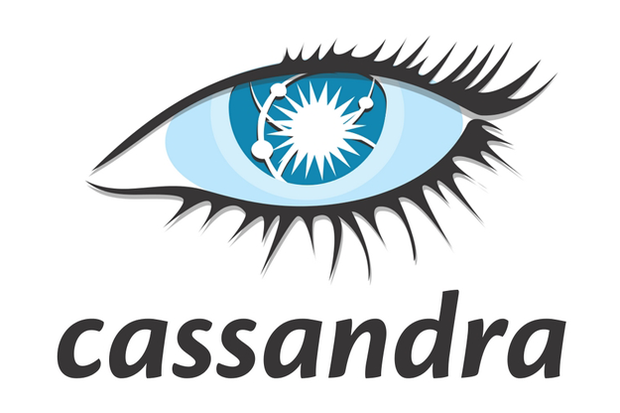
\includegraphics[width=10cm]{img/cassandra.png}
  \captionof{figure}{Cassandra}
\end{center}

Cassandra ban đầu được tạo ra bởi Facebook. Sau đó nó đã được tặng cho Quỹ Apache và tháng 2 năm 2010 và được nâng cấp lên thành dự án hàng đầu của Apache. Cassandra là một cơ sở dữ liệu phân tán kết hợp mô hình dữ liệu của Google Bigtable với thiết kế hệ thống phân tán như bản sao của Amazon Dynamo.\\

\textit{Đặc điểm và thế mạnh:}
\begin{itemize}
    \item Tính phân tán và không tập trung (distributed and decentralized): Khả năng phân chia dữ liệu thành nhiều phần, đặt trên nhiều node khác nhau trong khi người dùng vẫn nhận thấy dữ liệu này là một khối thống nhất.
    \item Tính mềm dẻo (elastic scalability): Hệ thống có thể dễ dàng mở rộng số node trong cluster để có thể phục vụ số lượng request lớn và rút bớt số node khi số lượng request giảm.
    \item Tính sẵn sàng cao (high availability): Dữ liệu được sao lưu thành nhiều bản và được chia thành nhiều node. Điều này mang lại khả năng đáp ứng ngay lập tức cho Cassandra khi Client thực hiện tác vụ đọc hay ghi bằng cách thực hiện trên bản sao gần nhất hoặc trên tất cả các bản sao.
    \item Tính nhất quán (consistance): trong Cassandra, dữ liệu sẽ nhất quán sau một khoảng thời gian nào đó chứ không phải được nhất quán ngay sau khi người dùng ghi dữ liệu
    \item Tính chấp nhận lỗi (fault tolerance): Do dữ liệu được sao chép thành nhiều bản trên các node của cluster nên kể cả khi dữ liệu ở một node nào đó bị lỗi, ta vẫn có thể truy xuất dữ liệu của mình trên một node khác.
    \item Tính hướng cột (column oriented key-value store): Các RDBMS hướng dòng (row-oriented) phải định nghĩa trước các cột (column) trong các bảng (table). Đối với Cassandra ta không phải làm điều đó, đơn giản là thêm vào bao nhiêu cột cũng được tùy theo nhu cầu của ta.
    \item Hiêụ năng cao (high performance): Cassandra được thiết kế riêng biệt từ sơ khai cho đến khi đầy đủ lợi ích cho máy đa luồng/đa lõi và được chạy trên hàng chục những máy được đặt trong các trung tâm dữ liệu với quy mô nhất quán và liên tục với hàng trăm terabyte dữ liệu.
\end{itemize}
\subsubsubsection{Redis}
\begin{center}
  \captionsetup{type=figure}
  
\includegraphics[width=10cm]{img/redis.png}
  \captionof{figure}{Redis}
\end{center}

Redis (REmote DIctionary Server) là một mã nguồn mở được dùng để lưu trữ dữ liệu có cấu trúc, có thể sử dụng như một cơ sở dữ liệu, bộ nhớ cache hay một message broker. Nó là hệ thống lưu trữ dữ liệu với dạng KEY-VALUE rất mạnh mẽ và phổ biến hiện nay.

Bên cạnh lưu trữ key-value trên RAM giúp tối ưu hiệu năng, Redis còn có cơ chế sao lưu dữ liệu trên đĩa cứng cho phép phục hồi dữ liệu khi gặp sự cố.\\

\textit{Đặc điểm:}
\begin{itemize}
    \item Đối tượng dữ liệu: Khác với RDMS như MySQL, hay PostgreSQL, Redis không có bảng. Redis lưu trữ data dưới dạng key-value.
    \item Khả năng mở rộng
    \item Lưu trữ trên bộ nhớ tạm: Không như các DBMS khác lưu trữ dữ liệu trên đĩa cứng, Redis lưu trữ dữ liệu trên RAM, và đương nhiên là thao tác đọc/ghi trên RAM.
\end{itemize}
\subsubsection{So sánh Relational Database và Non-Relational Database}
\begin{table}[H]
	    \centering
	    \begin{tabular}{|p{3cm}|p{6cm}|p{6cm}|}
	        \hline
	        &\textbf{Relational}&\textbf{Non-Relational}\\
	        \hline
	        Ngôn ngữ truy vấn&Ngôn ngữ truy vấn có cấu trúc &Truy vấn đối tượng: trực quan, chuyển một tài liệu để giải thích những gì bạn đang truy vấn\\
	        \hline
	        Kiểu dữ liệu&Lưu các kiểu dữ liệu được quy định&Có thể lưu bất kỳ loại dữ liệu nào\\
	        \hline
	        Khả năng mở rộng&Mở rộng thêm chiều dọc&Mở rộng theo chiều ngang\\
	        \hline
	        Hiển thị dữ liệu&Dưới dạng bảng và hàng&Dưới dạng JSON\\
	        \hline
	        Chi phí&Chi phí xây dựng và bảo trì cao&Khoảng 10\% so với Relational\\
	        \hline
	    \end{tabular}
	    \caption{So sánh cơ sở dữ liệu quan hệ và cơ sở dữ liệu phi quan hệ}
	\end{table}
	
	
Nội dung cần có:\\
SQL là gì, tính năng, thế mạnh, ...\\
|    SQL server (hình ảnh, là gì, đặc điểm, thế mạnh)\\
|    Oracle     (...)\\
|    MySQL      (...)\\
NoSQL là gì, tính năng, thế mạnh\\
|    MongoDB    (...)\\
|    Neo4j      (...)\\
|    Cassandra, tham khảo: \url{https://drive.google.com/open?id=1jM9vy5ExhZ1IROXV1J8gvoJrT_F64OYw}\\
So sánh SQL, NoSQL\\
m có thể làm 1 folder 7 rồi chia từng phần ra từng file cho dễ làmc